\documentclass[12pt]{article}

\usepackage{sbc-template}

\usepackage{graphicx,url}

\usepackage[brazil]{babel}   
%\usepackage[latin1]{inputenc}  
\usepackage[utf8]{inputenc}  
% UTF-8 encoding is recommended by ShareLaTex
\usepackage{verbatim}
     
\sloppy

\title{Making Sense de Desenvolvimento de Software e Tipos de Personalidade.}

\author{Jodiel Fabricio Dias dos Santos\inst{1} }


\address{Departamento de Informática -- Universidade Federal do Maranhão
  (UFMA)\\
  Cidade Universitária -- São Luís -- MA -- Brasil
  \email{jodielfabricio@gmail.com}
}

\begin{document} 

\maketitle
\begin{comment}
\begin{abstract}
  This meta-paper describes the style to be used in articles and short papers
  for SBC conferences. For papers in English, you should add just an abstract
  while for the papers in Portuguese, we also ask for an abstract in
  Portuguese (``resumo''). In both cases, abstracts should not have more than
  10 lines and must be in the first page of the paper.
\end{abstract}
\end{comment}

\begin{resumo} 
  Este artigo é um resumo do artigo \textit{"Making Sense of Software Development and Personality Types"} de autoria de Luiz Fernando Capretz, University of Western Ontario  e Faheem Ahmed, United Arab Emirates University \cite{capretz:2010}.
\end{resumo}


\section{Introdução}

Segundo a introdução do artigo, o software é um produto de certas atividades humanas como solução de problemas, processamento de informações cognitivas e interação social. Porém, as pessoas são mais complicadas e menos previsíveis do que os computadores, portanto, a complexidade da personalidade implica em uma complexa dinâmica que, em última análise, se torna parte integrante, ainda que negligenciada, do desenvolvimento de software.
Mais cedo ou mais tarde, as principais questões relevantes para a engenharia de software se resumem às pessoas envolvidas com a produção de software e seus traços de personalidade.


\section{Myers-Briggs Type Indicator } \label{sec:firstpage}

O indicador de Tipo Myers-Briggs  é uma ferramenta conhecido por medir e  compreender os tipos individuais de personalidade. Atualmente, está entre os indicadores mais populares usados no local de trabalho, estabelecendo quatro pares tridimensionais para avaliar os tipos de personalidade: 


\begin{itemize}
    \item Extroversão (E) e Introversão (I) - \textit{Extroversion (E) e Introversion (I)};
    \item Sentir (S) e Intuição (N) - \textit{Sensing (S) and Intuition (N)};
	\item Pensar (T) e Sentir (F) - \textit{Thinking (T) and Feeling (F)}
	\item Julgando (J) e Percebendo (P) - \textit{Judging (J) and Perceiving (P)}
\end{itemize}

 Ao usar esses quatro conjuntos de preferências, será selecionado um traço de cada par, para esboçar o tipo preferido de uma pessoa. 


\section{Mapeamento de Requisitos de Trabalho e Soft Skills para Tipos de Personalidade}\label{sec:figs}

De acordo com essa seção, \textit{Mapping Job Requirements and Soft Skills to Personality Types}, a engenharia de software é caracterizada por um conjunto de atividades que incluem \textbf{análise}, \textbf{design}, \textbf{programação}, \textbf{teste} e \textbf{manutenção do sistema}. Essas diferentes tarefas se combinam para atingir os objetivos de construção e operação de software.

\subsection{Análise de Sistema}

Nessa fase é enfatizado a identificação de componentes de alto nível em uma aplicação do mundo real e envolve a decomposição do sistema de software em seus módulos principais. 

É exigido, também, que o analista de sistemas determine as necessidades do usuário, considere os requisitos do cliente do sistema, compreenda os recursos essenciais do sistema e crie um modelo de aplicativo abstrato que atenda a esses requisitos.  
Portanto, ao nomear analistas de sistema, é preferível procurar por pessoas que possuam características extrovertidas (E) e de sentimento (F), veja a Figura~\ref{fig:figura1}.

\begin{figure}[!ht]
\centering
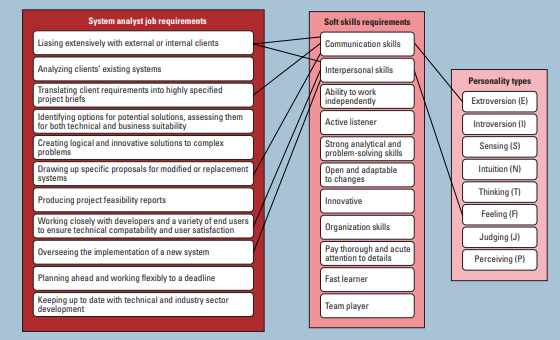
\includegraphics[width=.7\textwidth]{Capturar1.PNG}
\caption{Mapeamento de analistas de sistemas e suas habilidades para tipos de personalidade. Ao nomear um analista de sistema, é preferível procurar pessoas que possuam características extrovertidas (E) e de sentimento (F).}
\label{fig:figura1}
\end{figure}

\subsection{Design de Software}
Segundo os autores, "Design" é considerada uma palavra ambígua, pois embora haja grandes variações entre os princípios de design, é possível encontrar um conjunto comum de recursos que se aplicam ao design de qualquer artefato, contudo o design de software ainda seja um campo relativamente novo e longe de um consenso sobre seus princípios relevantes, ele exige a criatividade humana evidente em outras disciplinas, como arquitetura, marketing e design gráfico, em vez da construção estereotipada de outros campos da engenharia. 

Ainda segundo os autores, o design de software é considerado um processo exploratório, onde designer procura componentes testando vários esquemas para descobrir a maneira mais natural e razoável de refinar uma solução. E ainda design de software possa parecer uma tarefa fácil, na concepção de software grande e complexo, a identificação de componentes-chave é um esforço árduo e demorado. 

Logo repetições não são incomuns, já que um bom design geralmente leva várias iterações. Além disso, o número de iterações também depende do conhecimento e da experiência do designer no domínio do aplicativo.

Como mostra a Figura~\ref{fig:figura2}, os tipos N e T são altamente desejáveis para os projetistas de software, enquanto a percepção e o sentimento são apenas um pouco desejáveis. O Ps ajudaria a alcançar a melhor solução de design do que a primeira. Também é importante a capacidade de prever como os usuários se sentirão em relação ao design.
\begin{figure}[!ht]
\centering
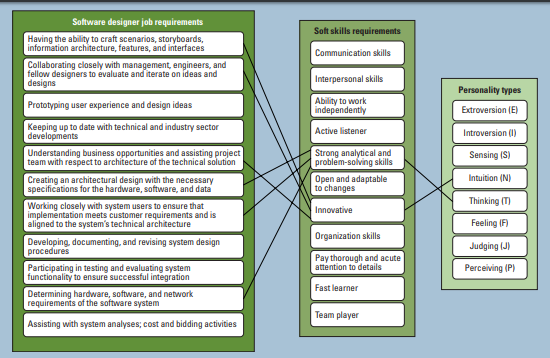
\includegraphics[width=.7\textwidth]{Capturar2.PNG}
\caption{Mapeamento de designers de software e suas habilidades para tipos de personalidade. Uma combinação de intuição (N) e pensamento (T) é primordial para prosperar no design.}
\label{fig:figura2}
\end{figure}

\subsection{Programação}
De acordo com autores, a programação envolve a tradução de uma versão refinada do design em programas. Essa fase envolve a identificação de estruturas de controle, variáveis relevantes e estruturas de dados, bem como uma compreensão detalhada da sintaxe e das especificidades de uma linguagem de programação. Os programadores devem seguir um processo de refinamento passo a passo iterativo que é principalmente de cima para baixo, largura primeiro. Logo, os programadores devem atender aos detalhes e manter um estilo de pensamento lógico e analítico. 

E segundo os autores, como mostra a Figura~\ref{fig:figura3}, os programadores que trabalham com as especificações dos designers precisam ser lógicos (Ts), prestar atenção aos detalhes (Ss) e ter a capacidade de trabalhar de forma independente (Is). Às vezes eles podem programar em pares ou até mesmo dentro de uma equipe, mas o núcleo da programação requer a capacidade de se concentrar e trabalhar sozinho por muitas horas. Dadas essas características, não é surpreendente que tantos engenheiros de software sejam ISTs.

\begin{figure}[!ht]
\centering
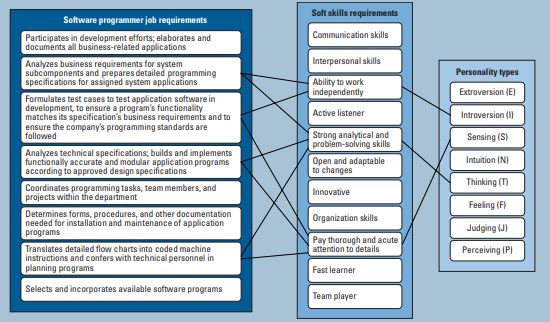
\includegraphics[width=.7\textwidth]{Capturar.PNG}
\caption{Mapeamento de programadores e suas habilidades para tipos de personalidade. A maioria dos programadores é introvertida (I), sensível (S), pensando (T).}
\label{fig:figura3}
\end{figure}

\subsection{Teste}
Para os autores, o estágio de teste não é a primeira vez que os defeitos são encontrados, pois podem surgir nas fases de análise e design do sistema, mas o foco principal do teste é encontrar o maior número possível de defeitos. O teste de unidade, verifica se um módulo funciona adequadamente com as várias entradas esperadas (e inesperadas) com base na especificação do módulo. Depois que as coletas de módulos são testadas em unidade, o próximo passo é garantir que as interfaces entre elas sejam bem definidas, o teste de integração. Finalmente, o teste do sistema é o processo de verificar e validar se o software inteiro funciona corretamente.

O teste requer atenção aos detalhes e muitas vezes é realizado por indivíduos que trabalham de forma independente, e a pressão para cumprir prazos e entregar o produto é enorme. Logo, precisão (S) e julgamento (J) são características altamente desejáveis. Em teoria, as pessoas S e J teriam mais sucesso na fase de testes, conforme ilustrado na Figura~\ref{fig:figura4}.
\begin{figure}[!ht]
\centering
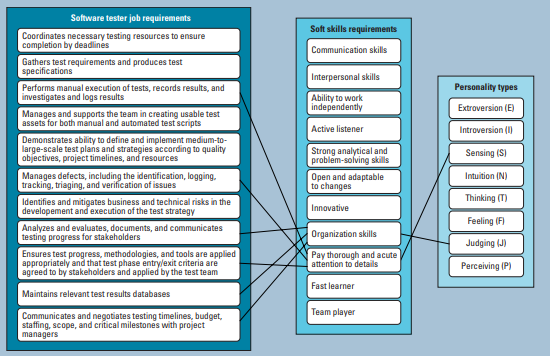
\includegraphics[width=.7\textwidth]{Capturar3.PNG}
\caption{Mapeando testadores e suas habilidades para tipos de personalidade. Em teoria, o sensoriamento (S) e o julgamento (J) das pessoas seriam mais bem-sucedidos na fase de testes.}
\label{fig:figura4}
\end{figure}
\subsection{Manutenção}
Para os autores, nessa fase o software está sujeito, normalmente, a mudanças contínuas depois de escrito e enquanto está operacional, indicando a necessidade de manter um sistema em evolução. 

Os projetos envolvendo pesquisa e desenvolvimento de ponta tendem a atrair mais pessoas, enquanto aqueles que têm tarefas relacionadas à manutenção e aprimoramento de sistemas de software tendem a atrair mais tipos S, que tendem a ser práticos, realistas e observadores, e os tipos P  gostam de explorar todas as possibilidades e, consequentemente, têm dificuldade em tomar decisões. 

Logo, a capacidade de resolver problemas e a abordagem prática dos SPs são um recurso para a manutenção porque essas pessoas gostam de resolver problemas práticos e aproveitar o desafio de corrigir.

A Figura~\ref{fig:figura5} exibe essas relações, destacando as qualidades do software
mantenedores.
\begin{figure}[!ht]
\centering
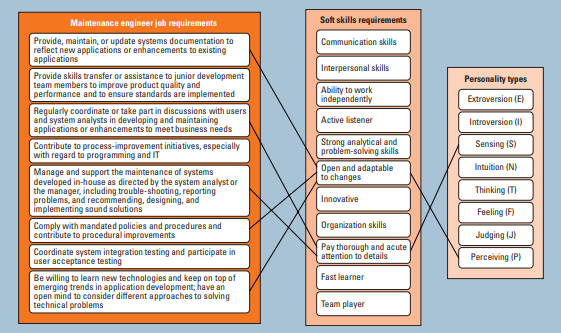
\includegraphics[width=.7\textwidth]{Capturar4.PNG}
\caption{Mapeamento de mantenedores e habilidades para tipos de personalidade. Detecção (S) e percepção (P) tipos são mais adequados para as tarefas orientadas a detalhes e constantes mudanças inerentes à manutenção de software.}
\label{fig:figura5}
\end{figure}
\section{Ciclo de Vida do Software mais Tipos de Personalidade}

Na ultima seção, os autores, mostram uma tabela, veja a Figura~\ref{fig:figura6}, com as cinco principais etapas de um modelo de ciclo de vida de software e propõe uma estrutura para conceituar os pontos em que um determinado tipo de personalidade poderia ter mais efeito. Assumimos que a análise, o projeto, a programação, o teste e a manutenção do sistema são os estágios que ocorrem com maior frequência em modelos de ciclo de vida de software bem aceitos, apesar de alguns modelos não considerarem alguns desses estágios ou outros. Independentemente do modelo usado, uma determinada dimensão de personalidade influencia cada um dos cinco estágios até certo ponto. 

A teoria por trás dos tipos de personalidade implica que cada um provavelmente afeta algumas fases do ciclo de vida do software mais do que outras. 

\begin{figure}[!ht]
\centering
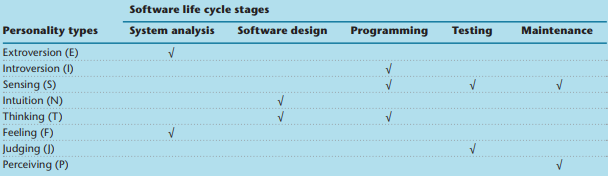
\includegraphics[width=.7\textwidth]{Capturar6.PNG}
\caption{Os tipos de personalidade com o impacto mais forte no ciclo de vida do software.}
\label{fig:figura6}
\end{figure}
\newpage
\section{References}

\bibliographystyle{sbc}
\bibliography{sbc-template}

\end{document}
